% Options for packages loaded elsewhere
\PassOptionsToPackage{unicode}{hyperref}
\PassOptionsToPackage{hyphens}{url}
\PassOptionsToPackage{dvipsnames,svgnames,x11names}{xcolor}
%
\documentclass[
]{article}
\usepackage{amsmath,amssymb}
\usepackage{setspace}
\usepackage{iftex}
\ifPDFTeX
  \usepackage[T1]{fontenc}
  \usepackage[utf8]{inputenc}
  \usepackage{textcomp} % provide euro and other symbols
\else % if luatex or xetex
  \usepackage{unicode-math} % this also loads fontspec
  \defaultfontfeatures{Scale=MatchLowercase}
  \defaultfontfeatures[\rmfamily]{Ligatures=TeX,Scale=1}
\fi
\usepackage{lmodern}
\ifPDFTeX\else
  % xetex/luatex font selection
\fi
% Use upquote if available, for straight quotes in verbatim environments
\IfFileExists{upquote.sty}{\usepackage{upquote}}{}
\IfFileExists{microtype.sty}{% use microtype if available
  \usepackage[]{microtype}
  \UseMicrotypeSet[protrusion]{basicmath} % disable protrusion for tt fonts
}{}
\makeatletter
\@ifundefined{KOMAClassName}{% if non-KOMA class
  \IfFileExists{parskip.sty}{%
    \usepackage{parskip}
  }{% else
    \setlength{\parindent}{0pt}
    \setlength{\parskip}{6pt plus 2pt minus 1pt}}
}{% if KOMA class
  \KOMAoptions{parskip=half}}
\makeatother
\usepackage{xcolor}
\usepackage[margin=1in]{geometry}
\usepackage{color}
\usepackage{fancyvrb}
\newcommand{\VerbBar}{|}
\newcommand{\VERB}{\Verb[commandchars=\\\{\}]}
\DefineVerbatimEnvironment{Highlighting}{Verbatim}{commandchars=\\\{\}}
% Add ',fontsize=\small' for more characters per line
\usepackage{framed}
\definecolor{shadecolor}{RGB}{248,248,248}
\newenvironment{Shaded}{\begin{snugshade}}{\end{snugshade}}
\newcommand{\AlertTok}[1]{\textcolor[rgb]{0.94,0.16,0.16}{#1}}
\newcommand{\AnnotationTok}[1]{\textcolor[rgb]{0.56,0.35,0.01}{\textbf{\textit{#1}}}}
\newcommand{\AttributeTok}[1]{\textcolor[rgb]{0.13,0.29,0.53}{#1}}
\newcommand{\BaseNTok}[1]{\textcolor[rgb]{0.00,0.00,0.81}{#1}}
\newcommand{\BuiltInTok}[1]{#1}
\newcommand{\CharTok}[1]{\textcolor[rgb]{0.31,0.60,0.02}{#1}}
\newcommand{\CommentTok}[1]{\textcolor[rgb]{0.56,0.35,0.01}{\textit{#1}}}
\newcommand{\CommentVarTok}[1]{\textcolor[rgb]{0.56,0.35,0.01}{\textbf{\textit{#1}}}}
\newcommand{\ConstantTok}[1]{\textcolor[rgb]{0.56,0.35,0.01}{#1}}
\newcommand{\ControlFlowTok}[1]{\textcolor[rgb]{0.13,0.29,0.53}{\textbf{#1}}}
\newcommand{\DataTypeTok}[1]{\textcolor[rgb]{0.13,0.29,0.53}{#1}}
\newcommand{\DecValTok}[1]{\textcolor[rgb]{0.00,0.00,0.81}{#1}}
\newcommand{\DocumentationTok}[1]{\textcolor[rgb]{0.56,0.35,0.01}{\textbf{\textit{#1}}}}
\newcommand{\ErrorTok}[1]{\textcolor[rgb]{0.64,0.00,0.00}{\textbf{#1}}}
\newcommand{\ExtensionTok}[1]{#1}
\newcommand{\FloatTok}[1]{\textcolor[rgb]{0.00,0.00,0.81}{#1}}
\newcommand{\FunctionTok}[1]{\textcolor[rgb]{0.13,0.29,0.53}{\textbf{#1}}}
\newcommand{\ImportTok}[1]{#1}
\newcommand{\InformationTok}[1]{\textcolor[rgb]{0.56,0.35,0.01}{\textbf{\textit{#1}}}}
\newcommand{\KeywordTok}[1]{\textcolor[rgb]{0.13,0.29,0.53}{\textbf{#1}}}
\newcommand{\NormalTok}[1]{#1}
\newcommand{\OperatorTok}[1]{\textcolor[rgb]{0.81,0.36,0.00}{\textbf{#1}}}
\newcommand{\OtherTok}[1]{\textcolor[rgb]{0.56,0.35,0.01}{#1}}
\newcommand{\PreprocessorTok}[1]{\textcolor[rgb]{0.56,0.35,0.01}{\textit{#1}}}
\newcommand{\RegionMarkerTok}[1]{#1}
\newcommand{\SpecialCharTok}[1]{\textcolor[rgb]{0.81,0.36,0.00}{\textbf{#1}}}
\newcommand{\SpecialStringTok}[1]{\textcolor[rgb]{0.31,0.60,0.02}{#1}}
\newcommand{\StringTok}[1]{\textcolor[rgb]{0.31,0.60,0.02}{#1}}
\newcommand{\VariableTok}[1]{\textcolor[rgb]{0.00,0.00,0.00}{#1}}
\newcommand{\VerbatimStringTok}[1]{\textcolor[rgb]{0.31,0.60,0.02}{#1}}
\newcommand{\WarningTok}[1]{\textcolor[rgb]{0.56,0.35,0.01}{\textbf{\textit{#1}}}}
\usepackage{longtable,booktabs,array}
\usepackage{calc} % for calculating minipage widths
% Correct order of tables after \paragraph or \subparagraph
\usepackage{etoolbox}
\makeatletter
\patchcmd\longtable{\par}{\if@noskipsec\mbox{}\fi\par}{}{}
\makeatother
% Allow footnotes in longtable head/foot
\IfFileExists{footnotehyper.sty}{\usepackage{footnotehyper}}{\usepackage{footnote}}
\makesavenoteenv{longtable}
\usepackage{graphicx}
\makeatletter
\def\maxwidth{\ifdim\Gin@nat@width>\linewidth\linewidth\else\Gin@nat@width\fi}
\def\maxheight{\ifdim\Gin@nat@height>\textheight\textheight\else\Gin@nat@height\fi}
\makeatother
% Scale images if necessary, so that they will not overflow the page
% margins by default, and it is still possible to overwrite the defaults
% using explicit options in \includegraphics[width, height, ...]{}
\setkeys{Gin}{width=\maxwidth,height=\maxheight,keepaspectratio}
% Set default figure placement to htbp
\makeatletter
\def\fps@figure{htbp}
\makeatother
\setlength{\emergencystretch}{3em} % prevent overfull lines
\providecommand{\tightlist}{%
  \setlength{\itemsep}{0pt}\setlength{\parskip}{0pt}}
\setcounter{secnumdepth}{-\maxdimen} % remove section numbering
\fontsize{12}{16}
\selectfont
\usepackage{lscape}
\usepackage{booktabs}
\usepackage{longtable}
\usepackage{array}
\usepackage{multirow}
\usepackage{wrapfig}
\usepackage{float}
\usepackage{colortbl}
\usepackage{pdflscape}
\usepackage{tabu}
\usepackage{threeparttable}
\usepackage{threeparttablex}
\usepackage[normalem]{ulem}
\usepackage{makecell}
\usepackage{xcolor}
\ifLuaTeX
  \usepackage{selnolig}  % disable illegal ligatures
\fi
\IfFileExists{bookmark.sty}{\usepackage{bookmark}}{\usepackage{hyperref}}
\IfFileExists{xurl.sty}{\usepackage{xurl}}{} % add URL line breaks if available
\urlstyle{same}
\hypersetup{
  pdftitle={Analisis Exploratorio de datos de la componente biológica},
  pdfauthor={Mardones, M; García, A.; Delgado, M.},
  colorlinks=true,
  linkcolor={blue},
  filecolor={Maroon},
  citecolor={Blue},
  urlcolor={Blue},
  pdfcreator={LaTeX via pandoc}}

\title{Analisis Exploratorio de datos de la componente biológica}
\usepackage{etoolbox}
\makeatletter
\providecommand{\subtitle}[1]{% add subtitle to \maketitle
  \apptocmd{\@title}{\par {\large #1 \par}}{}{}
}
\makeatother
\subtitle{Proyecto RECLAM}
\author{Mardones, M; García, A.; Delgado, M.}
\date{06 April, 2025}

\begin{document}
\maketitle

\setstretch{1.3}
\newpage
\tableofcontents
\newpage

\begin{Shaded}
\begin{Highlighting}[]
\FunctionTok{rm}\NormalTok{(}\AttributeTok{list =} \FunctionTok{ls}\NormalTok{())}
\NormalTok{knitr}\SpecialCharTok{::}\NormalTok{opts\_chunk}\SpecialCharTok{$}\FunctionTok{set}\NormalTok{(}\AttributeTok{echo =} \ConstantTok{FALSE}\NormalTok{,}
                      \AttributeTok{message =} \ConstantTok{FALSE}\NormalTok{,}
                      \AttributeTok{warning =} \ConstantTok{FALSE}\NormalTok{,}
                      \AttributeTok{fig.align =} \StringTok{\textquotesingle{}center\textquotesingle{}}\NormalTok{,}
                      \AttributeTok{dev =} \StringTok{\textquotesingle{}jpeg\textquotesingle{}}\NormalTok{,}
                      \AttributeTok{dpi =} \DecValTok{300}\NormalTok{, }
                      \AttributeTok{fig.align=}\StringTok{\textquotesingle{}center\textquotesingle{}}\NormalTok{)}
\CommentTok{\#XQuartz is a mess, put this in your onload to default to cairo instead}
\FunctionTok{options}\NormalTok{(}\AttributeTok{bitmapType =} \StringTok{"cairo"}\NormalTok{) }
\CommentTok{\# (https://github.com/tidyverse/ggplot2/issues/2655)}
\CommentTok{\# Lo mapas se hacen mas rapido}
\end{Highlighting}
\end{Shaded}

Datos faltantes o \texttt{NA}

\hypertarget{coquina}{%
\subsubsection{Coquina}\label{coquina}}

Regustros totalees por especie, mes, punto y replica.

\begin{center}\includegraphics{AED_Biologico_files/figure-latex/unnamed-chunk-6-1} \end{center}

Ahora vizualizamos las frecuencias de tallas de ambas especies a traves de los meses de muestreo

\begin{center}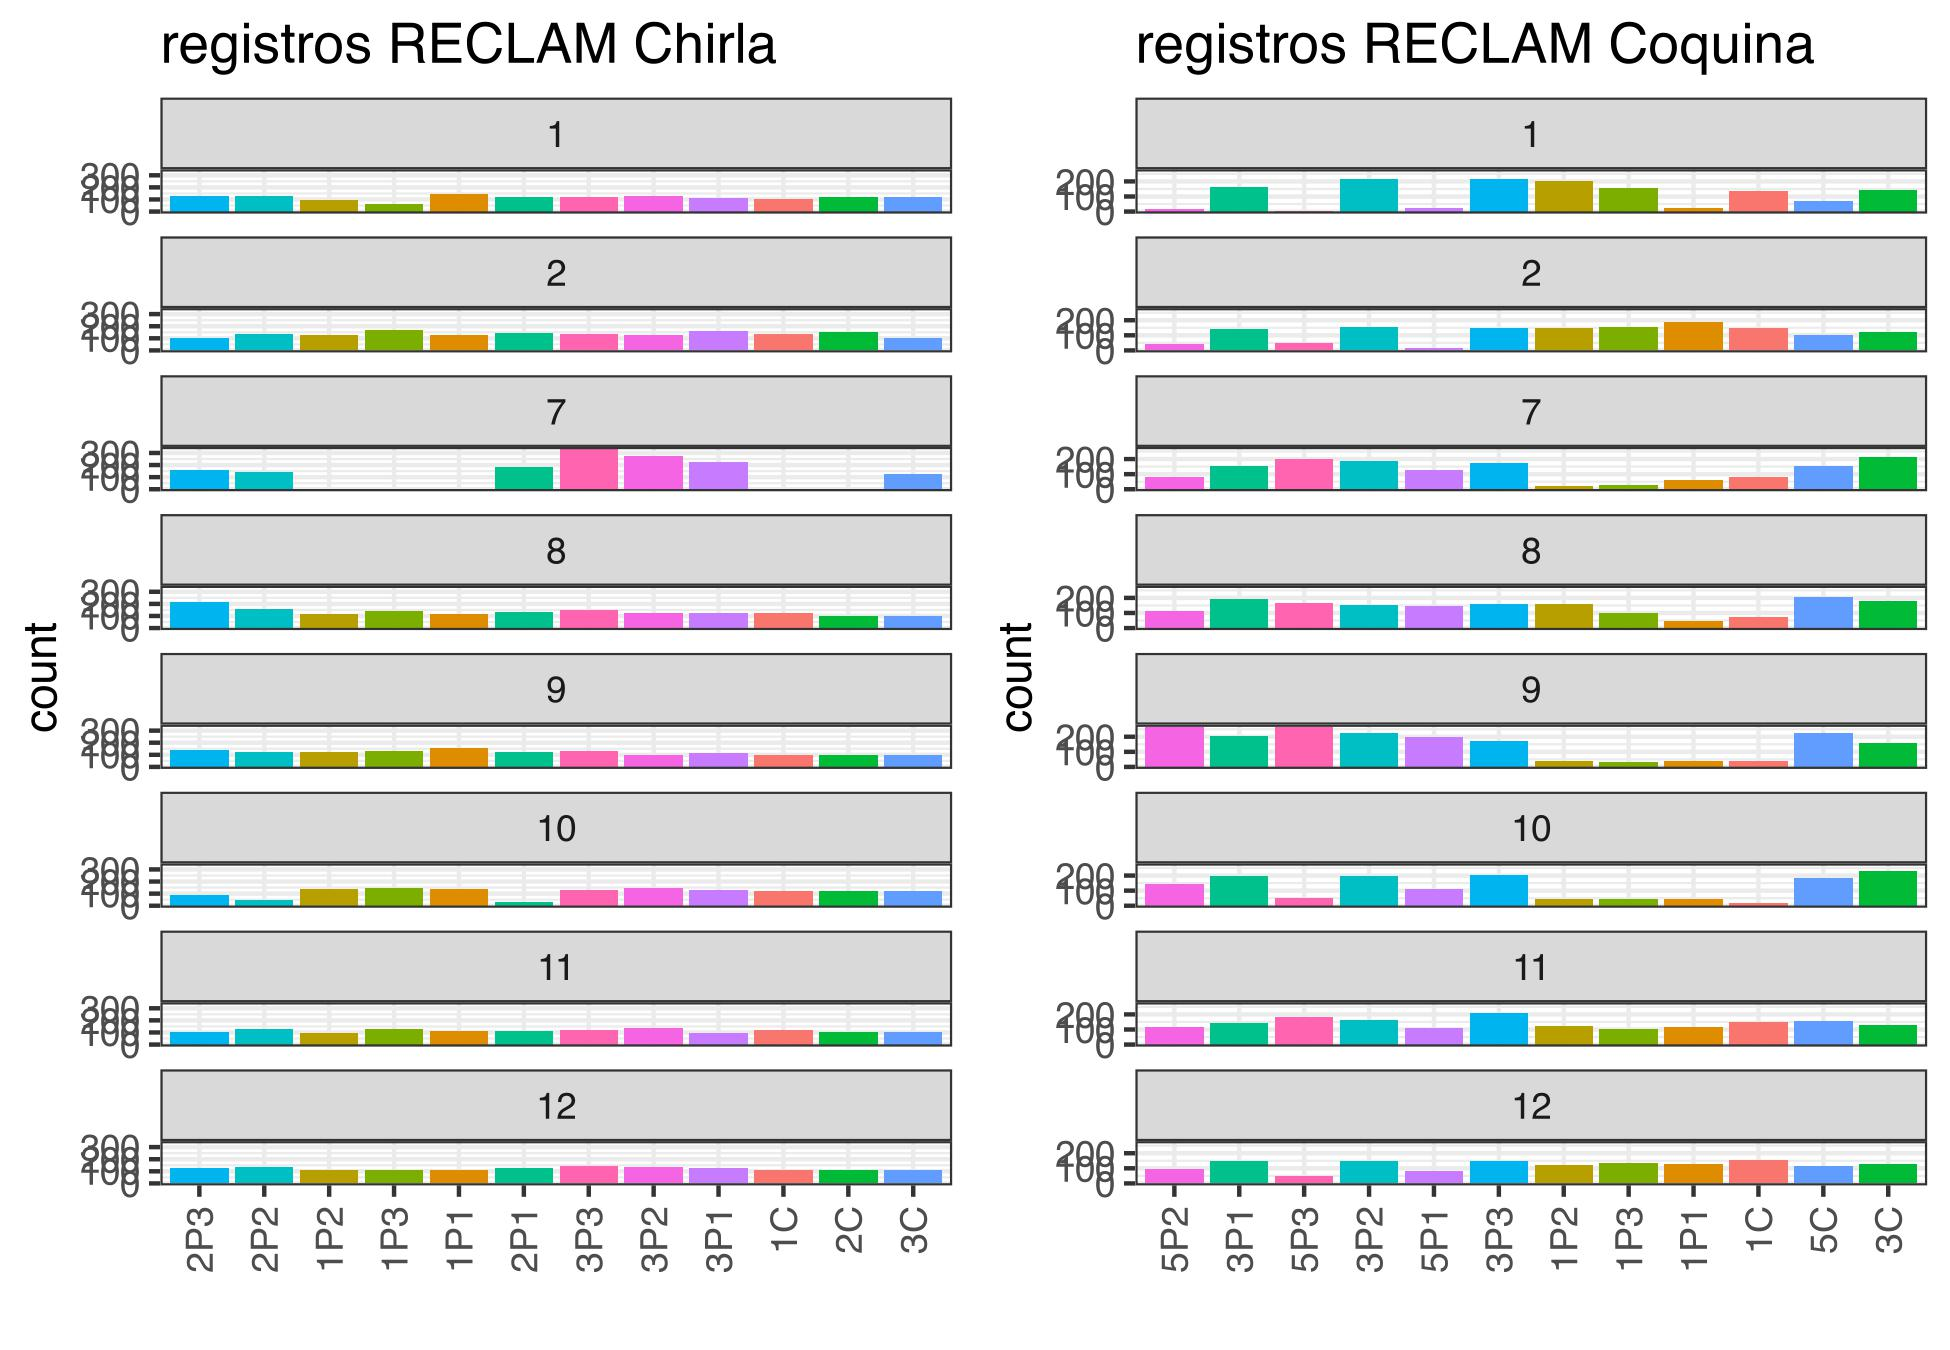
\includegraphics{AED_Biologico_files/figure-latex/unnamed-chunk-7-1} \end{center}

Tabla resumen de los individuos muestreados

\begin{table}

\caption{\label{tab:unnamed-chunk-9}Número de individuos muestreados de Chirla por mes y punto de muestreo}
\centering
\begin{tabular}[t]{ccccc}
\toprule
Ano & Mes & Especie & Punto & N° Individuos\\
\midrule
2025 & 1 & chirla & 1 & 406\\
2025 & 1 & chirla & 2 & 496\\
2025 & 1 & chirla & 3 & 470\\
2025 & 2 & chirla & 1 & 559\\
2025 & 2 & chirla & 2 & 533\\
\addlinespace
2025 & 2 & chirla & 3 & 522\\
2024 & 7 & chirla & 2 & 487\\
2024 & 7 & chirla & 3 & 958\\
2024 & 8 & chirla & 1 & 508\\
2024 & 8 & chirla & 2 & 603\\
\addlinespace
2024 & 8 & chirla & 3 & 501\\
2024 & 9 & chirla & 1 & 516\\
2024 & 9 & chirla & 2 & 486\\
2024 & 9 & chirla & 3 & 443\\
2024 & 10 & chirla & 1 & 540\\
\addlinespace
2024 & 10 & chirla & 2 & 283\\
2024 & 10 & chirla & 3 & 521\\
2024 & 11 & chirla & 1 & 451\\
2024 & 11 & chirla & 2 & 450\\
2024 & 11 & chirla & 3 & 460\\
\addlinespace
2024 & 12 & chirla & 1 & 441\\
2024 & 12 & chirla & 2 & 502\\
2024 & 12 & chirla & 3 & 519\\
\bottomrule
\end{tabular}
\end{table}

\begin{table}

\caption{\label{tab:unnamed-chunk-10}Número de individuos muestreados de Coquina por mes y punto de muestreo}
\centering
\begin{tabular}[t]{ccccc}
\toprule
Ano & Mes & Especie & Punto & N° Individuos\\
\midrule
2025 & 1 & coquina & 1 & 516\\
2025 & 1 & coquina & 3 & 737\\
2025 & 1 & coquina & 5 & 115\\
2025 & 2 & coquina & 1 & 640\\
2025 & 2 & coquina & 3 & 570\\
\addlinespace
2025 & 2 & coquina & 5 & 203\\
2024 & 7 & coquina & 1 & 193\\
2024 & 7 & coquina & 3 & 732\\
2024 & 7 & coquina & 5 & 557\\
2024 & 8 & coquina & 1 & 380\\
\addlinespace
2024 & 8 & coquina & 3 & 678\\
2024 & 8 & coquina & 5 & 635\\
2024 & 9 & coquina & 1 & 149\\
2024 & 9 & coquina & 3 & 763\\
2024 & 9 & coquina & 5 & 960\\
\addlinespace
2024 & 10 & coquina & 1 & 160\\
2024 & 10 & coquina & 3 & 831\\
2024 & 10 & coquina & 5 & 492\\
2024 & 11 & coquina & 1 & 495\\
2024 & 11 & coquina & 3 & 637\\
\addlinespace
2024 & 11 & coquina & 5 & 573\\
2024 & 12 & coquina & 1 & 541\\
2024 & 12 & coquina & 3 & 577\\
2024 & 12 & coquina & 5 & 348\\
\bottomrule
\end{tabular}
\end{table}

\hypertarget{relacion-talla-peso}{%
\subsection{Relacion Talla Peso}\label{relacion-talla-peso}}

Análisis recopilados desde este \href{https://rpubs.com/jdmaestre/366409}{Repo} and \href{http://derekogle.com/fishR/examples/oldFishRVignettes/LengthWeight.pdf}{this}
Estos datos fueron muestreados solo durante el mes de Junio 2024.

\begin{center}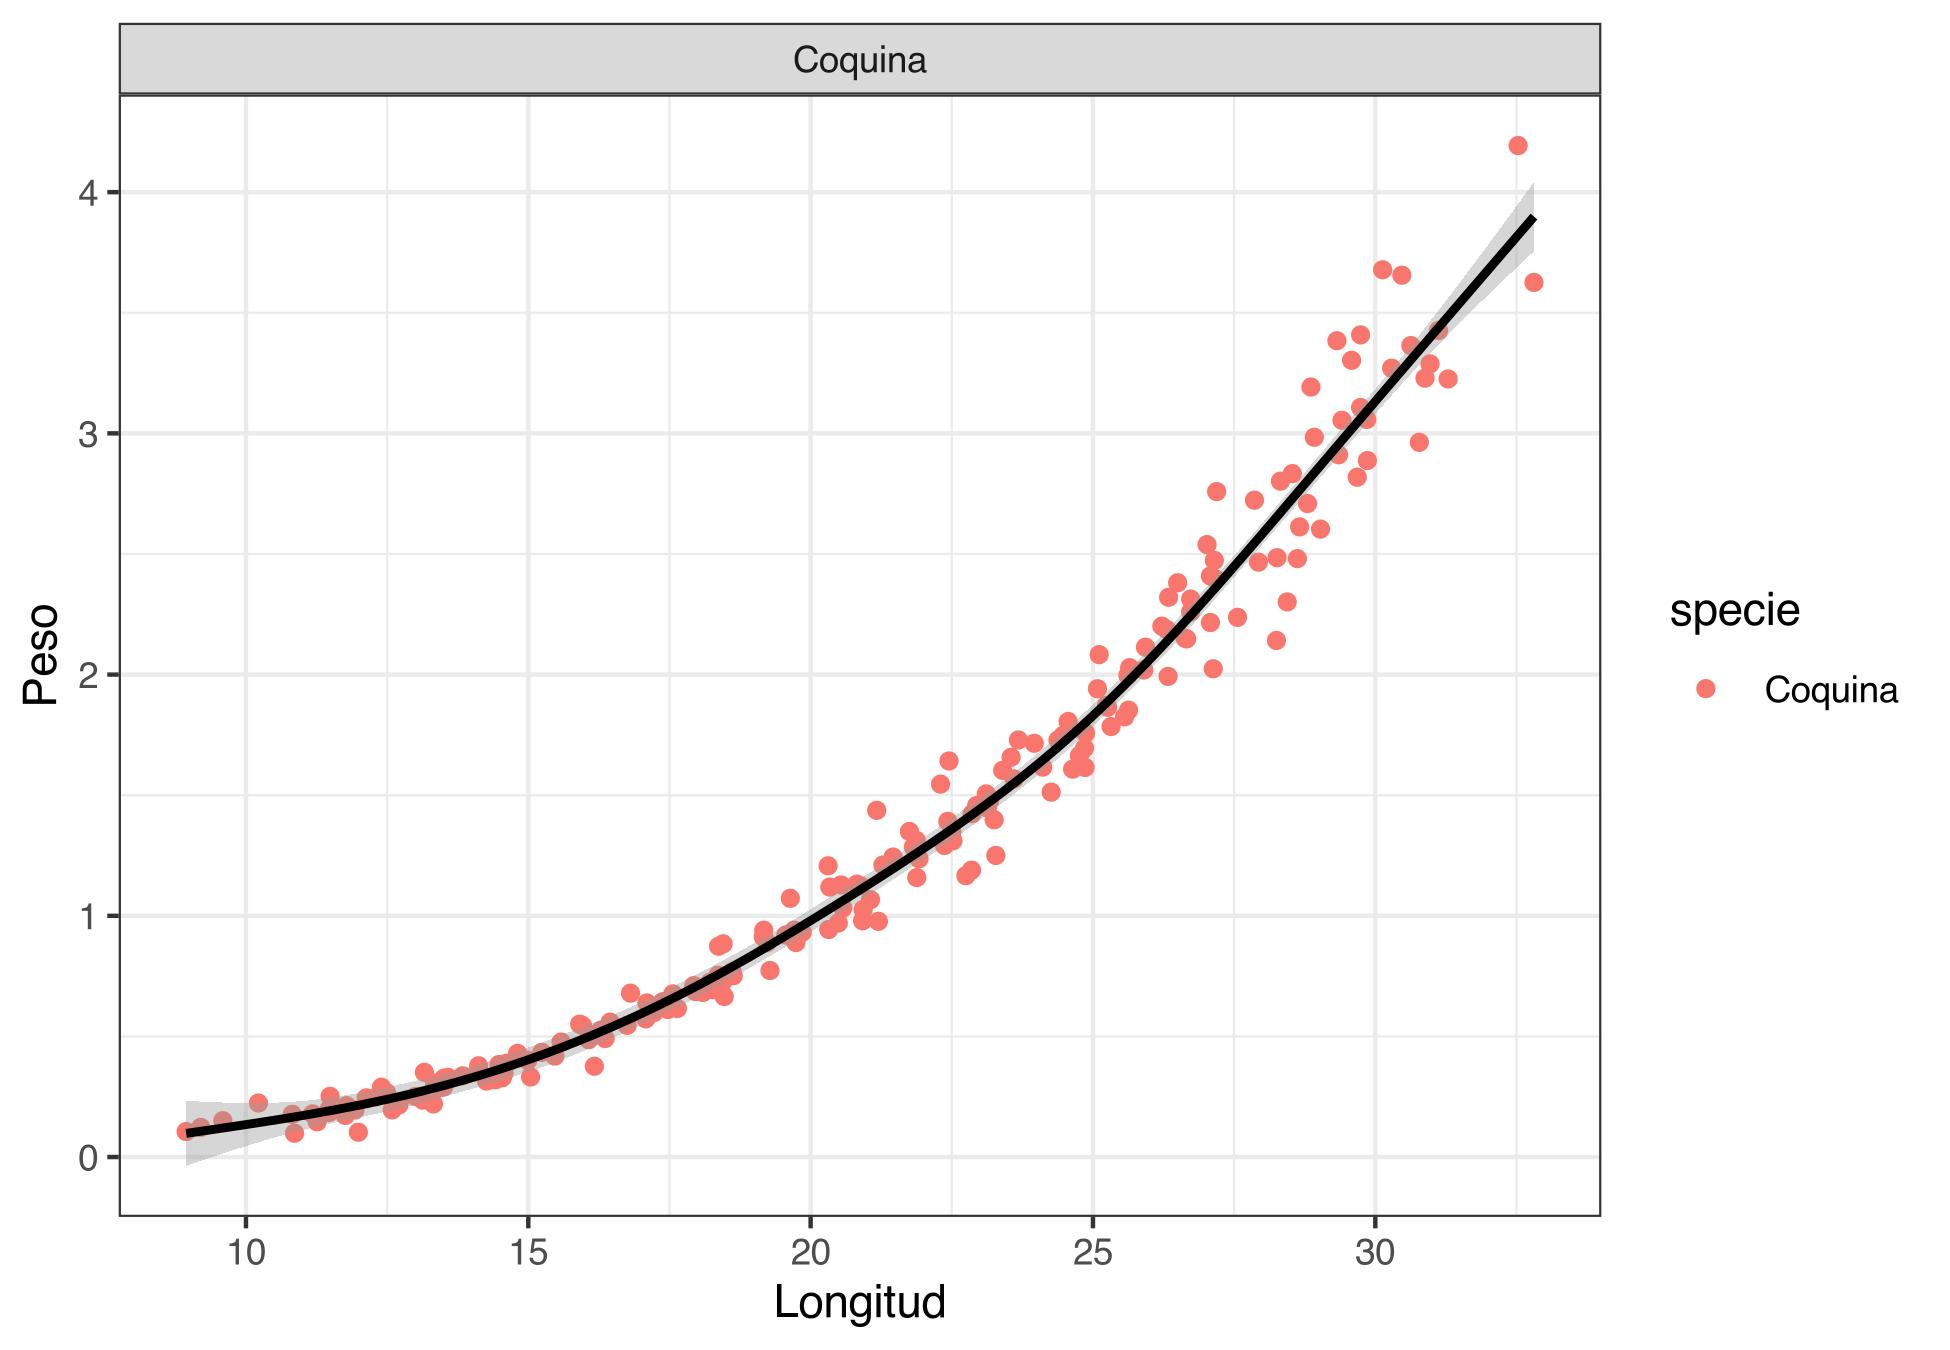
\includegraphics{AED_Biologico_files/figure-latex/unnamed-chunk-11-1} \end{center}

\begin{center}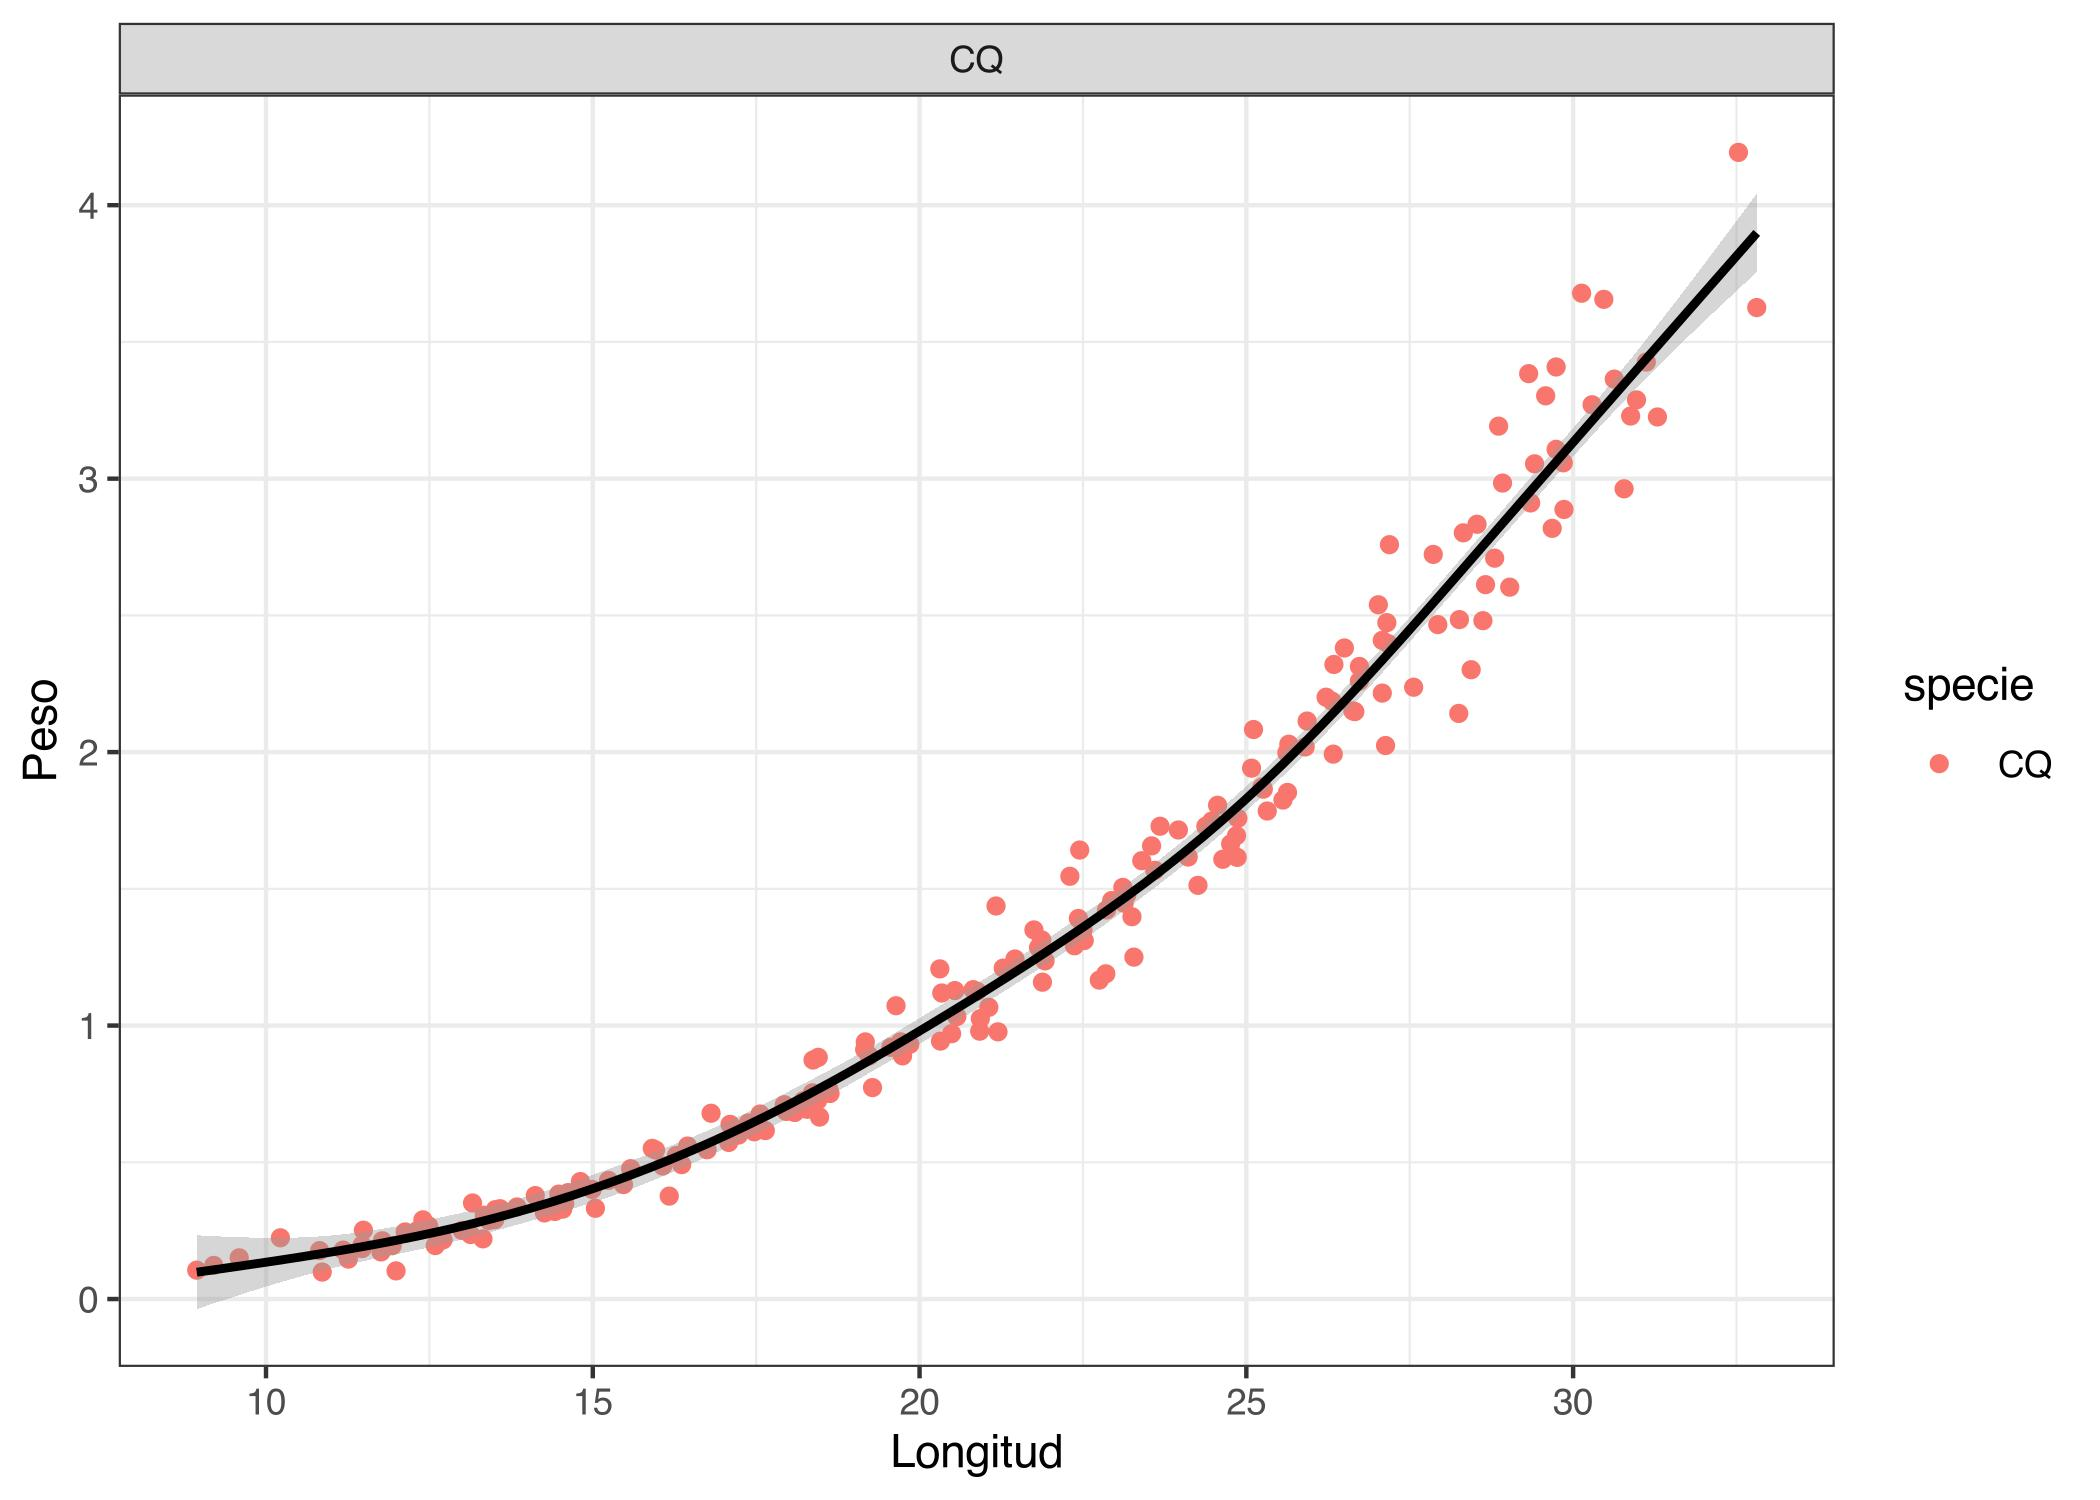
\includegraphics{AED_Biologico_files/figure-latex/unnamed-chunk-12-1} \end{center}

\begin{verbatim}
## Analysis of Variance Table
## 
## Response: log_Peso
##               Df Sum Sq Mean Sq F value    Pr(>F)    
## log_Longitud   1 160.68 160.682   10458 < 2.2e-16 ***
## Residuals    192   2.95   0.015                      
## ---
## Signif. codes:  0 '***' 0.001 '**' 0.01 '*' 0.05 '.' 0.1 ' ' 1
\end{verbatim}

\begin{verbatim}
##  (Intercept) log_Longitud 
##    -8.786510     2.917786
\end{verbatim}

\begin{verbatim}
## Intercepto (log): -8.78651
\end{verbatim}

\begin{verbatim}
## Pendiente (log): NA
\end{verbatim}

\begin{verbatim}
## Intercepto (absoluto): 0.0001527802
\end{verbatim}

\begin{center}\includegraphics{AED_Biologico_files/figure-latex/unnamed-chunk-14-1} \end{center}

\begin{center}\includegraphics{AED_Biologico_files/figure-latex/unnamed-chunk-14-2} \end{center}

\hypertarget{mapas}{%
\subsubsection{Mapas}\label{mapas}}

Preguntar a Alejandro si todos los ``Datos Lance'' tienen la misma Info. Por q no tiene Oct?

Unir base con \texttt{merge()}

(revisar!)

\begin{verbatim}
## # A tibble: 282,672 x 11
##     LONG FECHA                ZONA hoja  especie   ANO   MES   DIA PUNTO Latitud
##    <dbl> <dttm>              <dbl> <chr> <chr>   <dbl> <dbl> <int> <dbl>   <dbl>
##  1  26.6 2024-07-25 00:00:00     2 2P1   chirla   2024     7    25     2    36.6
##  2  26.6 2024-07-25 00:00:00     2 2P1   chirla   2024     7    25     2    36.6
##  3  26.6 2024-07-25 00:00:00     2 2P1   chirla   2024     7    25     2    36.6
##  4  26.6 2024-07-25 00:00:00     2 2P1   chirla   2024     7    25     2    36.6
##  5  26.6 2024-07-25 00:00:00     2 2P1   chirla   2024     7    25     2    36.6
##  6  26.6 2024-07-25 00:00:00     2 2P1   chirla   2024     7    25     2    36.6
##  7  26.6 2024-07-25 00:00:00     2 2P1   chirla   2024     7    25     2    36.6
##  8  26.6 2024-07-25 00:00:00     2 2P1   chirla   2024     7    25     2    36.5
##  9  28.0 2024-07-25 00:00:00     2 2P1   chirla   2024     7    25     2    36.6
## 10  28.0 2024-07-25 00:00:00     2 2P1   chirla   2024     7    25     2    36.6
## # i 282,662 more rows
## # i 1 more variable: Longitud <dbl>
\end{verbatim}

Leo un .shp

\begin{verbatim}
## Reading layer `costa_proyectada' from data source 
##   `/Users/mauriciomardones/IEO/IN_BENTOS/SHP_Chirla/costa_proyectada.shp' 
##   using driver `ESRI Shapefile'
## Simple feature collection with 10 features and 4 fields
## Geometry type: POLYGON
## Dimension:     XY
## Bounding box:  xmin: -34115.27 ymin: 3891271 xmax: 301588.8 ymax: 4173659
## Projected CRS: WGS_1984_Complex_UTM_Zone_30N
\end{verbatim}

\begin{verbatim}
## Reading layer `cuadrกculas_definitivo' from data source 
##   `/Users/mauriciomardones/IEO/IN_BENTOS/SHP_Chirla/cuadrกculas_definitivo.shp' 
##   using driver `ESRI Shapefile'
## Simple feature collection with 250 features and 1 field
## Geometry type: POLYGON
## Dimension:     XY
## Bounding box:  xmin: 109273.6 ymin: 4071852 xmax: 198073.5 ymax: 4125446
## Projected CRS: ETRS89 / UTM zone 30N
\end{verbatim}

\hypertarget{referencias}{%
\section{Referencias}\label{referencias}}

\end{document}
